\documentclass[a4paper, 12pt]{article}

\usepackage[italian]{babel}
\usepackage{verbatim}
\usepackage{graphicx}
\usepackage{float}
\usepackage[version=4]{mhchem}
\usepackage{subcaption}
\usepackage{pifont}
\usepackage[nottoc,numbib]{tocbibind}
\usepackage[style = chem-acs]{biblatex}


\renewbibmacro*{journal}{%
	\iffieldundef{shortjournal}
	{%
		\iffieldundef{journaltitle}
		{}
		{%
			\printtext[journaltitle]
			{%
				\printfield[titlecase]{journaltitle}%
				\setunit{\subtitlepunct}%
				\printfield[titlecase]{journalsubtitle}%
			}%
		}%
	}
	{\printtext[journaltitle]{\printfield[titlecase]{shortjournal}}}%
}

\bibliography{biblio.bib}


\oddsidemargin 30pt
\evensidemargin 20pt
\linespread{1.5}



\title{Sintesi di Composti d'Interesse Medico per il Trattamento del Morbo d'Alzheimer}
\author{
	Relatrice: Annamaria Deagostino
	\and
	Candidato: Lorenzo Castellino Test
}
\date{Anno Accademico 2017-2018}

\begin{document}
\pagenumbering{gobble}
\maketitle
\setcounter{page}{0}
\newpage
\tableofcontents
\newpage
\pagenumbering{arabic}

\section{Introduzione al Morbo d'Alzheimer}
La malattia di Alzheimer-Perusini, nota più comunemente come morbo d'Alzheimer (AD), è una tra le forme più diffuse al mondo di demenza senile. Dal punto di vista medico la patologia è definita come "disturbo neurocognitivo maggiore o lieve dovuto a malattia di  Alzheimer".\autocite{american_psychiatric_association_diagnostic_2013}
I sintomi associati sono differenti da individuo ad individuo, in generale nei pazienti riconosciuti si sono osservate:
\begin{enumerate}
	\item Perdita di memoria a breve termine.
	\item Difficoltà a concentrarsi, organizzarsi e di pianificazione.
	\item Difficoltà a seguire e/o formulare discorsi di senso compiuto.
	\item Difficoltà a giudicare distanze e spazi.
	\item Perdita di orientamento spaziale e temporale.
	\item Cambi repentini dell'umore.
	\item Allucinazioni visive.
\end{enumerate}
La demenza è una patologia di tipo progressivo, ovvero si ha un peggioramento dei sintomi col passare del tempo. La velocità di tale processo varia da persona a persona, tendenzialmente l'aspettativa media di vita successiva alla diagnosi della condizione va dai 3 ai 10 anni. \autocite{todd_survival_2013}

\subsection{L'Importanza della Ricerca}
L'incidenza dell'AD è in aumento tanto da individuare la ricerca di una cura come una delle sfide per il nuovo millennio: stando al World Alzheimer Report del 2018, stilato dall'Alzheimer's Disease International ovvero l'associazione internazionale per la lotta all'Alzheimer in stretta collaborazione con la World Health Organization, si stima che nel mondo circa 50 milioni di persone siano affette da demenza. Ciò si traduce in una spesa annua per il trattamento dei malati che rasenta il miliardo di dollari.

Con l'aumento dell'aspettativa media di vita si prevede che nel 2050 il numero di casi sarà il triplo di quello odierno e si prospetta una spesa doppia rispetto a quella attuale.\autocite{noauthor_world_2018}

Stando a queste previsioni 1'individuo su 85 nel 2050 sarà affetto da demenza.

L'individuazione delle cause che portano al presentarsi dell'AD è uno dei punti salienti della ricerca in campo medico e biochimico e molte sono state le ipotesi portate avanti a riguardo. Al momento una delle tesi più avvalorate e studiate è quella della formazione di aggregati proteici nel liquido cerebrospinale.

\subsection{\(\beta\)-Amiloidi e Placche Amiloidiche}
\label{sec:ab}
Con il termine \(\beta\)-amiloide (A\(\beta\)) si indica un frammento proteico insolubile non ramificato; tale nome è dovuto al fatto che al momento della scoperta, viste le sue proprietà si pensò ad una similitudine con le molecole d'amido benché dal punto di vista della composizione chimica non ci siano particolari somiglianze.\autocite{lennarz_encyclopedia_2004}

L'origine di queste strutture è legata all'azione congiunta di tre enzimi (\(\alpha\)-secretasi,\(\beta\)-secretasi e \(\gamma\)-secretasi) su di un substrato proteico noto come APP (Amyloid Precursor Protein). L'APP è una proteina trans-membrana di modeste dimensioni (circa 700 residui), viene trasportata lungo l'assone delle cellule neuronali ed il suo accumulo è focalizzato nei siti presinaptici. Il suo rilascio è regolato dall'attività elettrica cerebrale, si suppone infatti che abbia un ruolo fondamentale nella regolazione dell'eccitabilità neuronale.\autocite{mattson_cellular_1997}
La porzione che interessa la formazione di A\(\beta\) è situata nel dominio extracellulare dell'APP. Come si può osservare nella Figura~\ref{fig:app} i tre enzimi sopracitati agiscono in punti ben definiti e tra loro differenti della proteina; in particolare si osserva come l'azione dell'\(\alpha\)-secretasi non porti alla formazione del frammento A\(\beta\)  mentre l'azione dell'enzima \(\beta\) in congiunzione all'enzima \(\gamma\) generi la particolare sequenza.\autocite{goedert_century_2006}

\begin{figure}[H]
	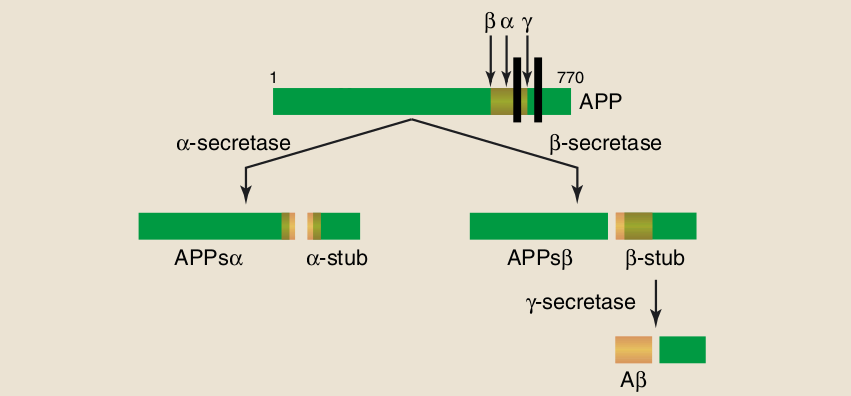
\includegraphics[width=\linewidth]{immagini/APP.png}
	\caption{Azione degli enzimi \(\alpha\)/\(\beta\)/\(\gamma\)-secretasi sul substrato APP.}
	\label{fig:app}
\end{figure}


I frammenti prodotti sono di due varietà che si differenziano per il numero di residui in essi contenuti, ecco quindi che possiamo distinguere i A\(\beta\)-40 e i A\(\beta\)-42 rispettivamente formati da 40 e 42 amminoacidi. Il rapporto tra le quantità prodotte delle due forme è di particolare importanza in quanto la A\(\beta\)-42 tende a formare oligomeri e fibrille più facilmente rispetto all’A\(\beta\)-40 molto probabilmente vista la minore solubilità data dai due residui idrofobici in più.\autocite{kepp_bioinorganic_2012, irvine_protein_2008}

La produzione di \(\beta\) in piccole quantità e un processo normale; delle funzioni osservate citiamo: \autocite{brothers_physiological_2018}

\begin{enumerate}
	\item Funzione antibatterica, antifunginea e antivirale.
	\item Soppressione tumorale.
	\item Meccanismo di riparazione di falle nella barriera emato-encefalica (azione simile alle piastrine nel sangue).
	\item Regolazione dell'attività sinaptica.
\end{enumerate}

Malgrado i benefici per l'organismo, una sovrapproduzione di A\(\beta\) o una sproporzione verso la forma contenente 42 residui associata ad uno smaltimento non efficace sembra essere una causa sufficiente per lo sviluppo precoce del Morbo d’Alzheimer. \autocite{irvine_protein_2008}
La demolizione avviene parzialmente direttamente nel cervello, come abbiamo infatti visto l'\(\alpha\)-secretasi effettivamente rende innocui i frammenti amiloidici scindendoli in due porzioni inerti; ma una gran parte di essa è delegata ad enzimi demolitori presenti nel fegato. La diffusione del frammento proteico insolubile è regolata dal recettore proteico LRP1 il cui processo di endocitosi è contrastato dall'azione del recettore antagonista RAGE (Figura \ref{fig:bbb}).\autocite{lillis_beyond_2005, dries_extracting_2012}

\begin{figure}[H]
	\centering
	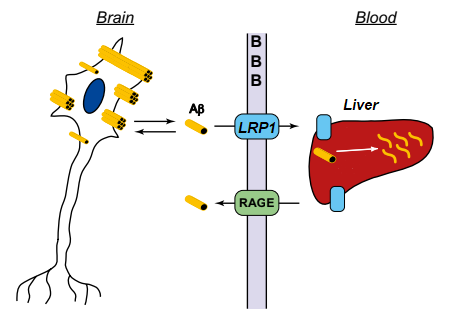
\includegraphics[width=.8\linewidth]{immagini/bbb.png}
	\caption{Fenomeno di migrazione dei A\(\beta\) attraverso la barriera emato-encefalica (BBB) verso il fegato ed effetto inverso legato al recettore RAGE).}
	\label{fig:bbb}
\end{figure}

All'aumento della concentrazione di A\(\beta\) nel liquido cerebrospinale è infatti associata la tendenza alla formazione di aggregati proteici più grandi ed insolubili detti comunemente "placche" o "fibrille".
L'accumulo di queste altera la chimica delle sinapsi, rallentando la trasmissione tra neuroni fino al punto di impedirla, causando così infine la morte della cellula.

Altre evidenze sperimentali mostrano come l’organismo, a causa di invecchiamento o condizioni di stress, ad esempio la mancanza di sonno, risulti meno efficiente nella demolizione, amplificando gli effetti di accumulo nel liquido cerebrospinale.

Un'altra delle ipotesi presenta come motivo primo dell'aggregazione in placche dei frammenti A\(\beta\) la presenza di concentrazioni elevate di ioni metallici nel liquido cerebrospinale. I metalli presi in esame sono Ferro, Rame e Zinco le cui concentrazioni, superato il valore di circa 10\textsuperscript{-7}  M diventano rilevanti per quanto riguarda la possibilità di essere complessati dai A\(\beta\) causando una tossicità diretta o fungendo come centri iniziatori di polimerizzazione per le fibrille amiloidiche.\autocite{kepp_bioinorganic_2012}

\section{Strategie d'Intervento}
Visto il complesso sistema che regola la comparsa dei A\(\beta\) vien da sé che anche i metodi per cercare di limitarne la presenza o gli effetti sull'organismo saranno altrettanto variegati.

Le metodologie d'intervento studiate nel panorama della ricerca biomedica sono le più disparate. Limitandoci solo a tecniche la cui azione è incentrata direttamente sui A\(\beta\) o sui loro effetti sull'organismo possiamo citare:\autocite{kumar_review_2015}
\begin{enumerate}
	\item Mitigazione del trasporto dei A\(\beta\) agendo sull'attività dei recettori LRP1 e RAGE.
	\item Modulazione degli enzimi responsabili della formazione di A\(\beta\), in particolare modulando la demolizione tramite l'\(\alpha\)-secretasi o inibendo la produzione per mezzo della \(\beta\)-secretasi.
	\item Limitazione dell'aggregazione dei A\(\beta\) in oligomeri e placche.
	\item Vaccinazione con oligomeri di A\(\beta\), l'intento è quello di stimolare una risposta immunitaria all'accumularsi degli aggregati amiloidici.
	\item Modulazione della neurotrasmissione in modo da limitare l'effetto d'inibizione delle sinapsi.
	\item Mitigazione degli effetti da stress ossidativo.
\end{enumerate}

Nella seguente trattazione ci limiteremo a presentarne alcuni con esempi di composti potenzialmente interessanti dal punto di vista farmacologico soffermandoci infine in maniera più estesa su di un possibile processo di sintesi per ognuno di essi.
La discussione verterà in particolare attorno a due composti la cui azione potrebbe limitare e rallentare la neurodegenerazione nelle Sezioni \ref{sec:resv} e \ref{sec:curc}, per poi affrontare invece una possibile tecnica mirata a prevenire il presentarsi dell'AD nella Sezione \ref{sec:byp}.

\section{Resveratrolo}
\label{sec:resv}
Il Resveratrolo (3,4,5'-triidrossil-trans-stilbene) è un polifenolo presente in molte piante, in particolare nella buccia e nei semi dell'uva. La sua funzione primaria nei vegetali è quella di fitoalessina, ovvero una risposta naturale nei confronti di infezioni batteriche e funginee. Alcuni studi hanno evidenziato anche diverse altre funzioni biologiche importanti come antiossidante, antinfiammatorio, fitoestrogeno e cardioprotettore.

Anche nel campo delle malattie neurodegenerative il Resveratrolo presenta alcune potenzialità; sono stati osservati effetti di riduzione dell'aggregazione dei A\(\beta\) e una modulazione della neurotrasmissione mediata da Acetilcolina.

Dal punto di vista medico tale molecola è quindi un potenziale candidato per lo sviluppo di farmaci in grado di mitigare l'effetto della demenza. \autocite{jabir_cholinesterase_2018}

\subsection{La Molecola}
La molecola, la cui struttura è presentata in Figura \ref{fig:resveratrolo}, è presente in natura in quantità apprezzabili in una grande varietà di piante come ad esempio le già citate bucce degli acini d'uva, ma anche in frutti con guscio, arachidi e alcune bacche. L'estrazione dai vegetali che contengono il composto, per quanto di facile realizzazione, non è sufficiente a coprire la domanda che le applicazioni in campo medico e di ricerca richiedono. Risulta quindi chiaro che lo sviluppo di un metodo di sintesi efficace e con bassi costi di realizzazione sia fondamentale per rendere economicamente valida la possibilità di impiego come medicinale della molecola.
\begin{figure}[H]
	\centering
	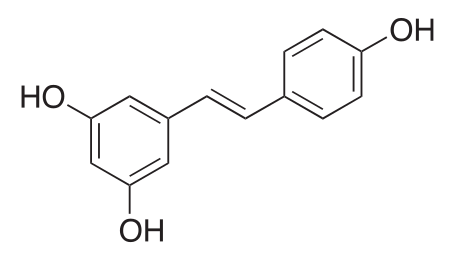
\includegraphics[width=.5\linewidth]{immagini/resveratrolo.png}
	\caption{Struttura molecolare del Resveratrolo.}
	\label{fig:resveratrolo}
\end{figure}
Oltre alla sintesi del Resveratrolo verranno presentate anche modifiche strutturali la cui presenza sembra avere un impatto positivo sull'azione del composto in casi di AD.

\subsection{Sintesi Mediante Accoppiamento Heck-Mizoroki}
Uno dei metodi più semplici ed efficaci per sintetizzare la molecola di Resveratrolo può essere realizzato mediante un accoppiamento di Heck-Mizoroki.
La reazione di accoppiamento di Heck-Mizoroki è un processo sintetico Palladio catalizzato che si prefigge come obbiettivo la formazione di un nuovo legame carbonio-carbonio a partire da un gruppo arilico, allilico o vinilico alogeno sostituito e un alchene. L'alchene può essere mono o disostituito e dal punto di vista elettronico può presentarsi come elettronricco, elettrondeficiente o neutro. Il ciclo catalitico, rappresentato schematicamente in Figura \ref{fig:heck}, viene condotto in condizioni basiche; tendenzialmente le basi utilizzate possono essere \ce{Et3N}, \ce{NaOAc} oppure \ce{Na2CO3} in ambiente acquoso. \autocite{clayden_organic_2012}
Nel caso del Resveratrolo la sintesi a partire da reagenti commerciali è composta di due passaggi sintetici.

\begin{figure}[H]
	\centering
	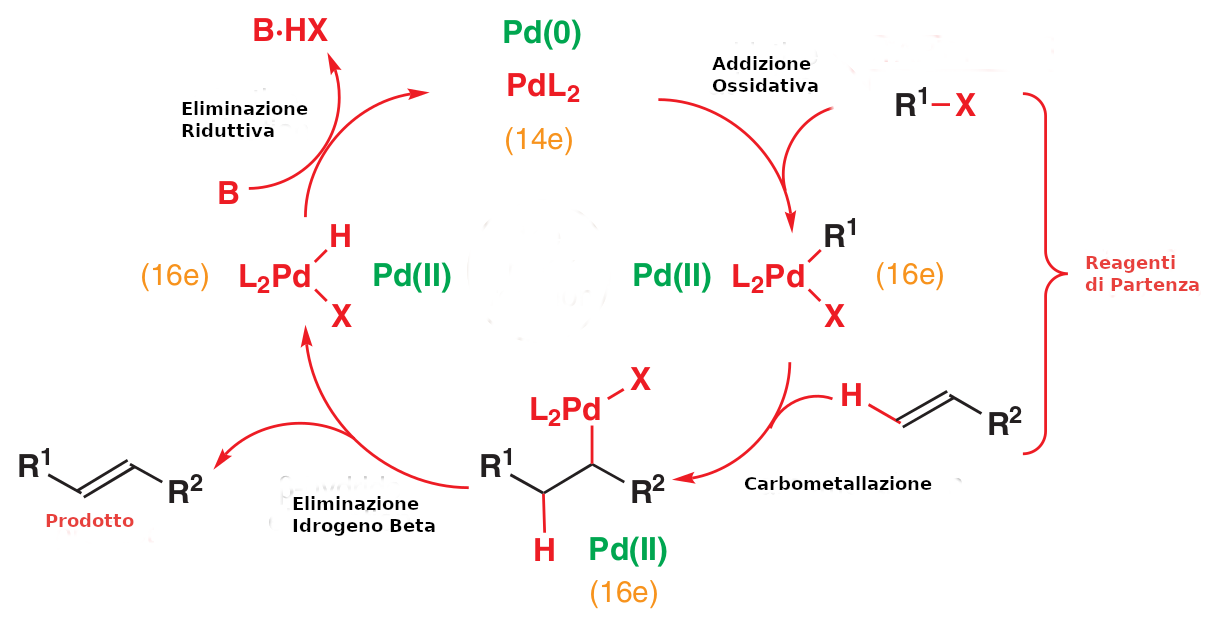
\includegraphics[width=\linewidth]{immagini/heck.png}
	\caption{Rappresentazione schematica del ciclo catalitico coinvolto in una reazione di Heck-Mizoroki.}
	\label{fig:heck}
\end{figure}

\subsubsection{Reazione di Accoppiamento}
I reagenti di partenza utilizzati per l'accoppiamento sono lo 1-iodo-3,5-dimetossibenzene ed il 4-metossistirene. Il catalizzatore impiegato è un catalizzatore di palladio nanoparticellare disperso su di un supporto di argilla laponite.

La preparazione di tale dispersione viene effettuata riducendo il \ce{H2PdCl4} con etanolo in presenza di polivinilpirrolidone (PVP), il ruolo del polimero è quello di permettere una migliore dispersione degli atomi di Palladio al fine di ottenere una riduzione delle dimensioni delle nanoparticelle desiderate.

Le nanoparticelle di Palladio stabilizzate sul PVP sono quindi impregnate sulla laponite lavorando in condizioni di atmosfera inerte ed utilizzando come solvente diclorometano. \autocite{martinez_extremely_2015}

Il catalizzatore così ottenuto può essere maneggiato ed utilizzato senza particolari precauzioni in reazioni atte a promuovere formazioni di legami carbonio-carbonio.

La reazione è riassunta nella Figura \ref{fig:h-m_resveratrolo}.

\begin{figure}[H]
	\centering
	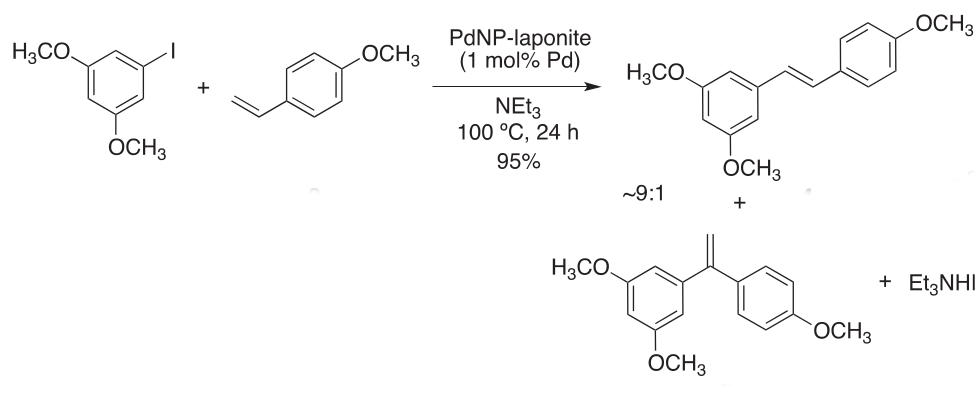
\includegraphics[width=\linewidth]{immagini/h-m_resveratrolo.png}
	\caption{Reazione di accoppiamento tra lo 1-iodo-3,5-dimetossibenzene ed il 4-metossistirene.}
	\label{fig:h-m_resveratrolo}
\end{figure}

Il ciclo catalitico è composto da quattro passaggi:
\begin{enumerate}
	\item Il catalizzatore \ce{PdL2} subisce addizione ossidativa da parte dello 1-iodo-3,5-dimetossibenzene passando da stato Pd(0) a Pd(II), ovvero da un complesso metallico a 14 elettroni ad uno a 16 elettroni.
	\item Il 4-metossistirene da carbometallazione legandosi al complesso metallico, si osserva l'inserimento del dimetossibenzene.
	\item Eliminando l'idrogeno \(\beta\) i due isomeri ottenibili originati dal nuovo legame carbonio-carbonio vengono allontanati dal catalizzatore.
	\item La base forte in soluzione, in questo caso la \ce{NEt3}, ripristina il catalizzatore con Pd(0) restituendo come prodotto il composto \ce{Et3NHI}.
\end{enumerate}

La quantità di Palladio residua nei prodotti, misurata mediante analisi ad ICP-MS, risulta essere molto bassa. In una catalisi eterogenea di questo tipo è stato dimostrato che le nanoparticelle di Palladio fungono puramente da riserve di Pd(0) e che quindi la pressoché totale assenza di tracce di Palladio al termine della reazione è molto probabilmente dovuta ad un riformarsi di nanoparticelle metalliche al termine del ciclo catalitico (secondo un meccanismo di reazione "a boomerang") o ad una deposizione delle stesse sul supporto inorganico impiegato.

Il catalizzatore eterogeneo presenta alcuni vantaggi rispetto ad un equivalente catalizzatore omogeneo; come si può osservare in Figura \ref{fig:perc_cata_resv} il catalizzatore depositato sulla fase inorganica presenta ottime rese nei primi dieci usi. Il sottoprodotto \ce{Et3NHI} inoltre viene allontanato dal grezzo durante il decorso della reazione per deposizione dello stesso sul supporto di Laponite. D'altra parte occorre tenere conto che dopo svariati cicli di reazione la quantità di sale depositato tende ad eccedere la quantità di nanoparticelle di Palladio presenti sul supporto inficiando quindi sulla resa di reazione. Il problema è risolvibile però in maniera relativamente facile attraverso il trattamento ad alta temperatura dell'argilla di supporto. Il Trietilenammonioioduro a 550 $^\circ$C in presenza di aria subisce un processo di calcinazione; il solido restante presenta ancora una buona attività come catalizzatore nelle reazioni e può essere impiegato nuovamente per almeno tre cicli reattivi senza perdere le sue proprietà.

\begin{figure}[H]
	\centering
	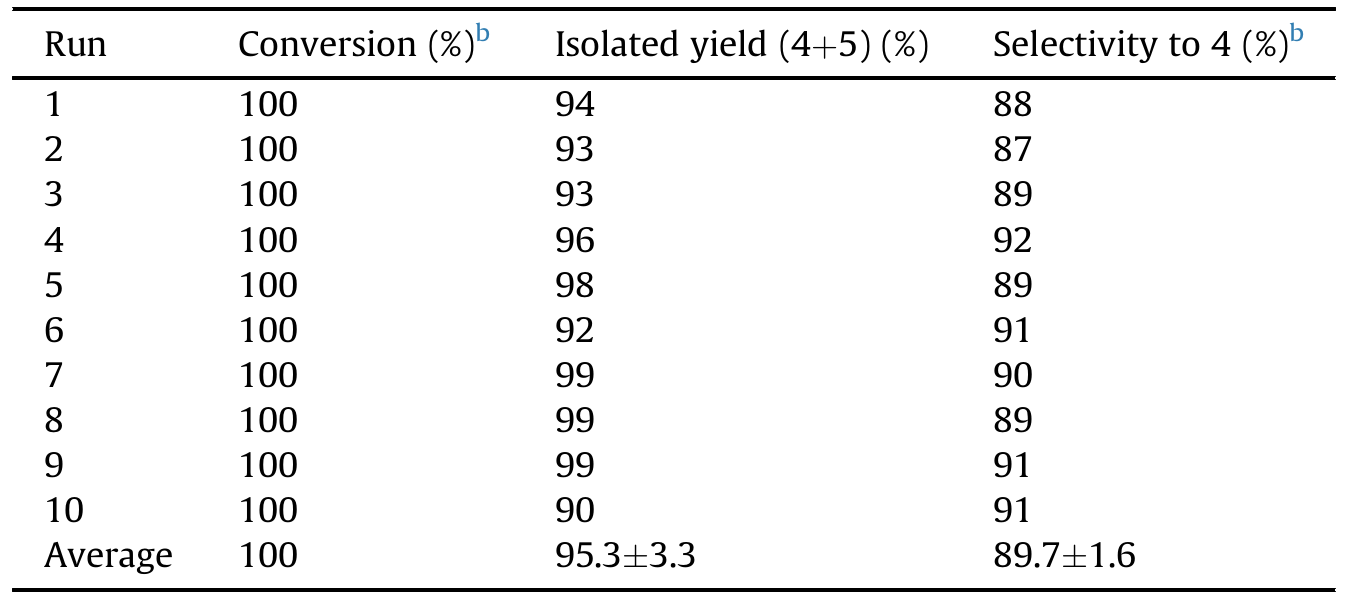
\includegraphics[width=\linewidth]{immagini/perc_cata_resv.png}
	\caption{Rese di reazione per dieci cicli catalitici successivi eseguiti utilizzando lo stesso catalizzatore. 4 = 3,4,5'-triidrossil-trans-stilbene; 5 = 3,4,5'-triidrossil-cis-stilbene}
	\label{fig:perc_cata_resv}
\end{figure}

\subsubsection{Eliminazione della Protezione Metilica}
Ai fini di ottenere la molecola di Resveratrolo è necessario rimuovere la protezione metilica presente sui gruppi metossi per ottenere sui fenoli dei gruppi idrossilici.

Tale passo sintetico è facilmente realizzabile mediante l'uso di un acido di Lewis come il Tribromuro di Bromo in diclorometano. La reazione è presentata in Figura \ref{fig:deprot_resveratrolo}; come si può osservare le rese per questo tipo di processo sono alte ed il processo è di facile realizzazione. \autocite{alejandro_v._martinez_expedient_2017}

\begin{figure}[H]
	\centering
	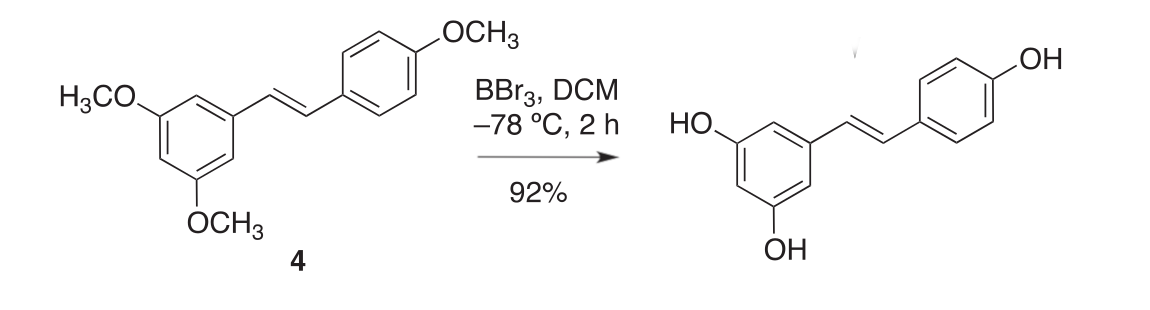
\includegraphics[width=\linewidth]{immagini/deprot_resveratrolo.png}
	\caption{Reazione di deprotezione del gruppo idrossilico sulla molecola sintetizzata.}
	\label{fig:deprot_resveratrolo}
\end{figure}

\subsection{Effetti delle Molecole Sintetizzate}
\label{effetti_resveratrolo}
L'azione medicinale del Resveratrolo in pazienti affetti da AD è principalmente attribuibile a due componenti:

\begin{enumerate}
	\item Regolazione dell'attività neuronale.
	\item Diminuzione della citotossicità dei A\(\beta\).
\end{enumerate}

La regolazione dell'attività neuronale è da ricondursi all'azione che la molecola ha nei confronti dell'enzima Acetilcolinesterasi (AChE). Tale enzima scinde l'Acetilcolina, noto neurotrasmettitore, in Colina e Acido Acetico dopo che la molecola ha partecipato alla sinapsi tra neuroni.

\begin{figure}[H]
	\centering
	\begin{subfigure}[b]{0.3\linewidth}
		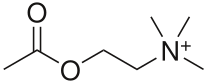
\includegraphics[width=\linewidth]{immagini/acetilcolina.png}
		\subcaption{Acetilcolina}
	\end{subfigure}
	~
	\begin{subfigure}[b]{0.3\linewidth}
		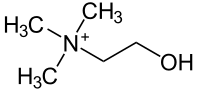
\includegraphics[width=\linewidth]{immagini/colina.png}
		\subcaption{Colina}
	\end{subfigure}
	\label{fig:coline}
\end{figure}

In casi di AD la neurotrasmissione viene ridotta in efficacia a causa dell'accumulo degli aggregati amiloidici più volte citati; ecco quindi che la normale azione dell'AChE risulta essere troppo aggressiva, e la molecola di Acetilcolina rischia di essere scissa prima di aver stimolato il neurone recettore.

Il Resveratrolo funge da inibitore dell'AChE, in particolare l'inibizione è promossa da alcuni suoi oligomeri, come ad esempio la Vitisina A e lo Heyneanol A le cui strutture sono riportate in Figura \ref{fig:oly_resveratrolo}.

\begin{figure}[H]
	\centering
	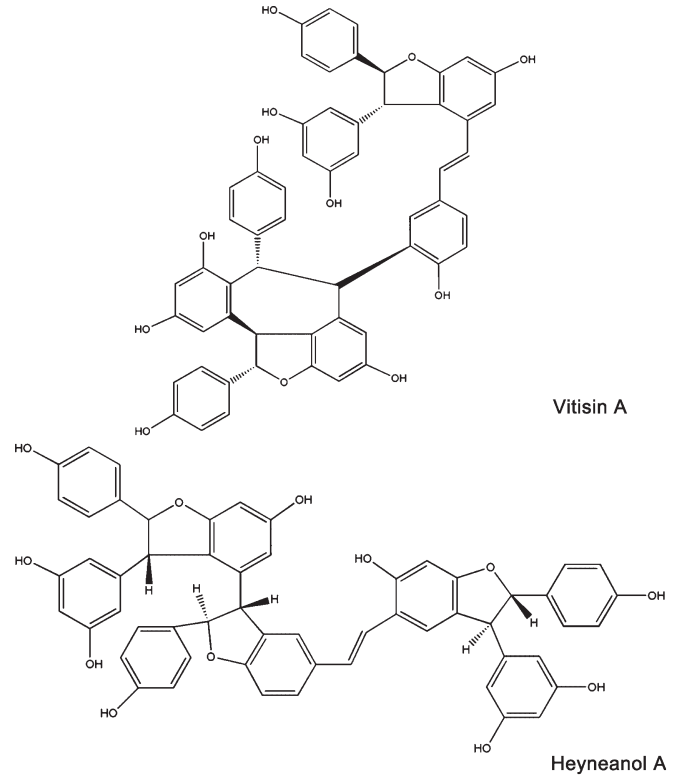
\includegraphics[width=\linewidth]{immagini/oly_resveratrolo.png}
	\caption{Struttura degli oligomeri del Resveratrolo.}
	\label{fig:oly_resveratrolo}
\end{figure}

L'azione di tali composti in presenza dell'enzima è stata osservata mediante un biotest HPLC; tale test prevede la raccolta del segnale originato da un rivelatore UV-vis in coda al sistema cromatografico. Nel caso particolare in questione due segnali a 16 minuti e a 23 minuti d'eluizione sono stati riconosciuti come indicatori dell'inibizione dell'attività enzimatica. L'esperimento è stato condotto in assenza e a concentrazioni variabili dei due tetrameri; l'inibizione è stata valutata per rapporto tra le intensità dei segnali caratteristici appena citati.  I risultati sono riportati in Figura \ref{fig:risache_resveratrolo}. Come si può osservare entrambe le molecole hanno dimostrato una buona capacità di diminuire l'attività dell'AChE con una discreta dipendenza dalla concentrazione.

\begin{figure}[H]
	\centering
	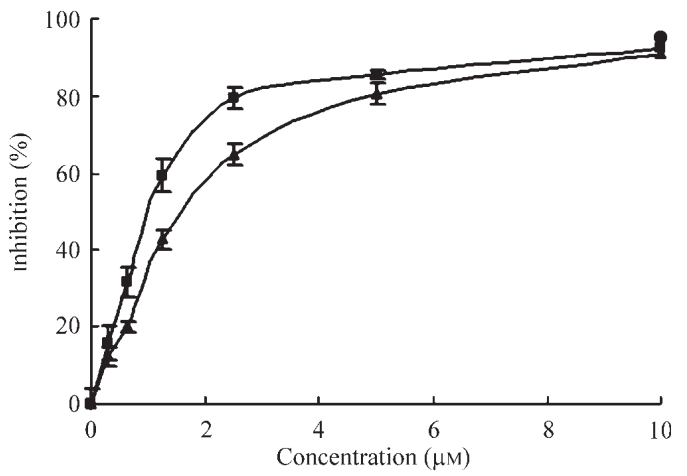
\includegraphics[width=.9\linewidth]{immagini/risache_resveratrolo.png}
	\caption{Percentuale d'inibizione dell'attività dell'enzima AChE per i composti Vitisina A (\ding{110}) e Heyneanol A (\ding{115}). }
	\label{fig:risache_resveratrolo}
\end{figure}

Altro paramentro importante nella regolazione dell'attività enzimatica è la proprietà della molecola di non andare ad agire in maniera equamente aggressiva su enzimi simili all'AChE come la Butirrilcolinesterai (BuChE). Per valutare ciò è stato eseguito un biotest del tutto analogo a quello sopra presentato. I risultati sono riportati in Figura \ref{fig:risbuche_resveratrolo}. Si può osservare come l'azione dei due composti, a differenza dell'inibizione dell'AChE, risulti significativamente asimmetrica; più precisamente i valori di IC\textsubscript{50} per la Vitisina A e per l'Heyneanol A corrispondono rispettivamente a 4,41 $\mu$M e 1,75 $\mu$M. La selettività nei confronti dell'AChE risulta quindi maggiore per la Vitisina A, candidandola di fatto come un buon inibitore selettivo. \autocite{jang_inhibition_2008}

\begin{figure}[H]
	\centering
	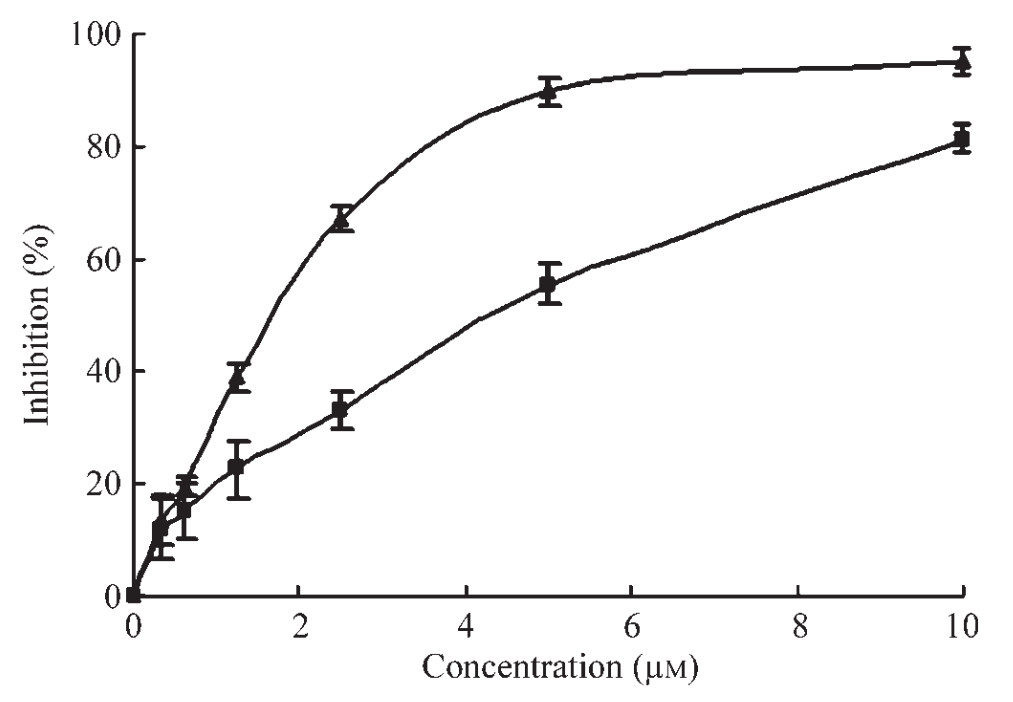
\includegraphics[width=.9\linewidth]{immagini/risbuche_resveratrolo.png}
	\caption{Percentuale d'inibizione dell'attività dell'enzima BuChE per i composti Vitisina A (\ding{110}) e Heyneanol A (\ding{115}). }
	\label{fig:risbuche_resveratrolo}
\end{figure}

Il secondo metodo d'azione del Resveratrolo è legato, come anticipato sopra, ad una diminuzione della tossicità dei depositi proteici di A\(\beta\). In particolare l'azione osservata è una diminuzione nel numero di fenomeni di  apoptosi nelle cellule neuronali e un ridursi in concentrazione di specie reattive ossidanti (ROI) nocive per l'organismo la cui formazione è promossa dalle fibrille stesse.

Gli esperimenti condotti ai fini di avvalorare l'importanza dal punto di vista medico del composto sono stati eseguiti utilizzando cellule della serie PC12, cellule di feocromocitoma di ratto.

Come si può osservare nella Figura \ref{fig:apo_resveratrolo} l'aggiunta di Resveratrolo in presenza di A\(\beta\) ha dimostrato una diminuzione della mortalità cellulare dopo un periodo d'incubazione di 36h. Il dato è ancora più evidente se si osserva la frammentazione del DNA evidenziata nella stessa figura nei pannelli (d), (e) ed (f).

\begin{figure}[H]
	\centering
	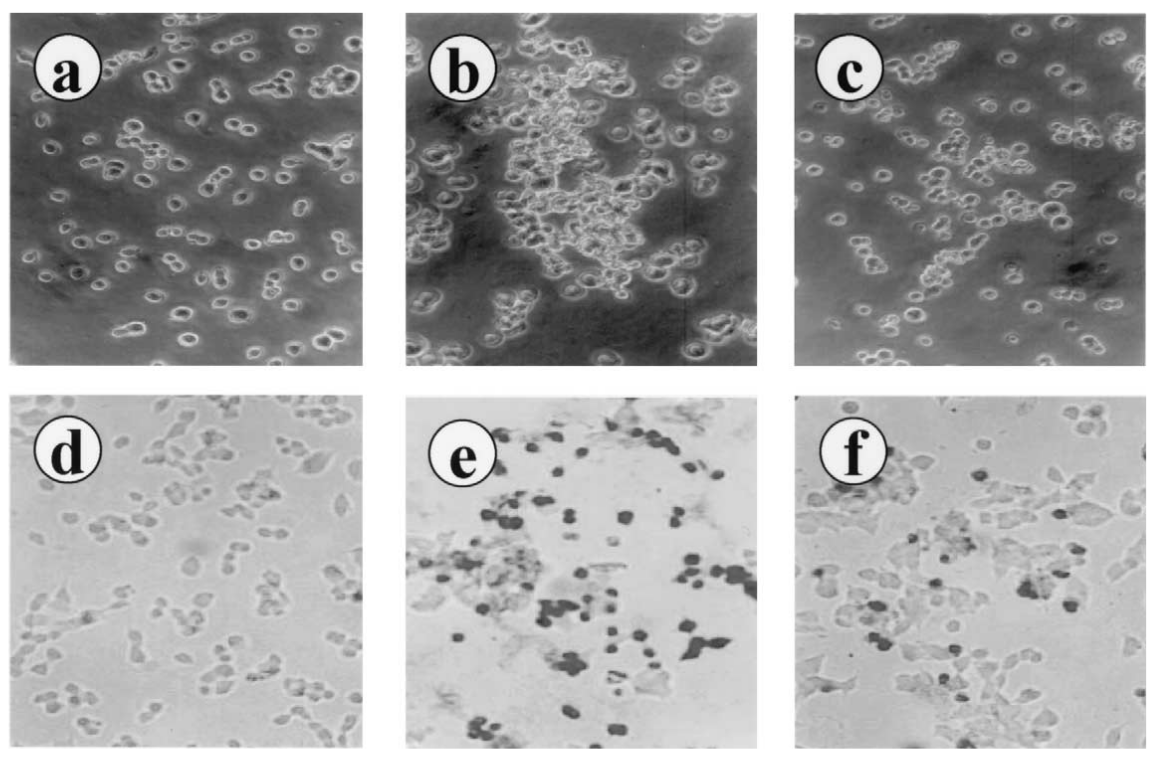
\includegraphics[width=.9\linewidth]{immagini/apo_resveratrolo.png}
	\caption{Immagini al microscopio di cellule PC12 (a) senza alcun trattamento; (b) in soluzione 50$\mu$M di A\(\beta\) dopo 36h; (c) in soluzione come (b) con l'aggiunta di Resveratrolo in concentrazione 25$\mu$M. Nei tre ingrandimenti inferiori sono invece state evidenziate le frammentazioni del DNA nelle stesse condizioni di (a), (b) e (c).}
	\label{fig:apo_resveratrolo}
\end{figure}

In Figura \ref{fig:roi_resveratrolo} sono invece riportati i dati relativi alle concentrazioni di ROI nelle cellule. Le immagini sono il risultato dell'osservazione della soluzione di cellule nello spettro UV in presenza di Diclorofluoresceina (DCF), un composto che emette radiazione UV in presenza di perossidi. Si può notare come la quantità di specie ossidanti risulti ridotta in maniera significativa in presenza di Resveratrolo. \autocite{jang_protective_2003}

\begin{figure}[H]
	\centering
	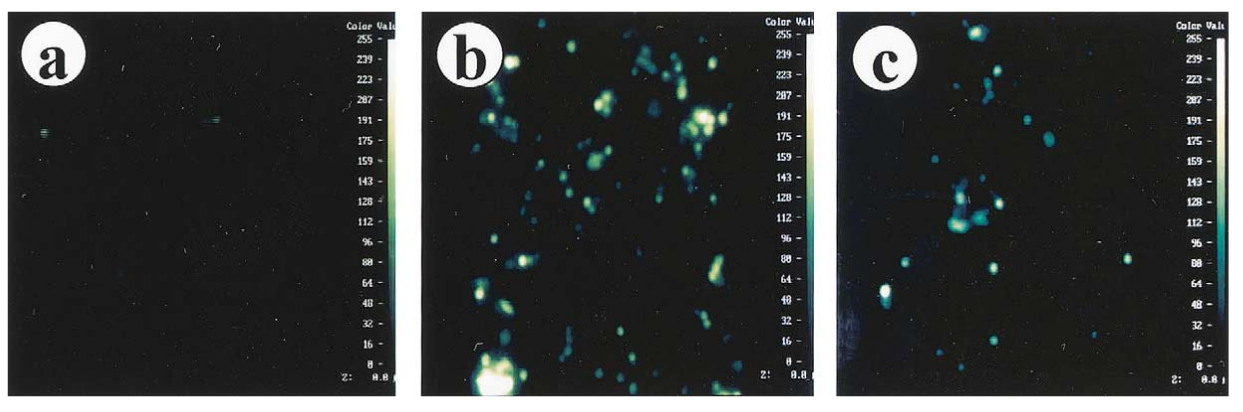
\includegraphics[width=.9\linewidth]{immagini/roi_resveratrolo.png}
	\caption{Livelli di perossidi intracellulari evidenziati tramite fluorescenza DCF (a) nessun trattamento; (b) A\(\beta\) 25$\mu$M; (c) A\(\beta\) 25$\mu$M + Resveratrolo 25$\mu$M.}
	\label{fig:roi_resveratrolo}
\end{figure}

\section{Curcumina}
\label{sec:curc}
La Curcumina ((1E,6E)-1,7-bis-(4-idrossi-3-metossifenil)-epta-1,6-dien- 3,5-dione) è la principale componente polifenolica della Curcuma; tale molecola è impiegata nel trattamento di molteplici malattia umane, il suo primo uso in questo frangente può essere ricondotto addirittura all'antica medicina cinese.

Ai giorni nostri in campo medico trova applicazioni nel tentativo di curare pazienti affetti da mieloma, psoriasi, cancro pancreatico, sindrome mielodisplasica e AD.

\subsection{La Molecola}
In Figura \ref{fig:curcumina} è presentata la formula di struttura della Curcumina. L'azione della molecola nei confronti dell'AD è attribuibile a diversi fattori:

\begin{enumerate}
	\item Mitigazione dell'aggregazione dei A\(\beta\).
	\item Azione di potenziamento cognitivo.
	\item Moderata inibizione dell'enzima AChE.
\end{enumerate}

Tutti questi effetti sono legati alla particolare struttura della molecola; la presenza di due anelli aromatici e la loro distanza relativa possono interagire con la struttura quaternaria  e i siti periferici dell'AChE. Sempre le funzionalità aromatiche presenti sono responsabili dell'effetto sulla formazione di placche amiloidiche.

I vantaggi derivati dall'uso della Curcumina come punto di partenza per lo sviluppo di rimedio all'AD sono la sua elevata permeabilità della barriera emato-encefalica e la relativa semplicità con cui è possibile effettuare modificazioni sulla sua struttura rendendola quindi un ottimo scheletro di partenza per la sintesi di farmaci più sofisticati. \autocite{jabir_cholinesterase_2018, jiang_traditional_2017}

\begin{figure}[H]
	\centering
	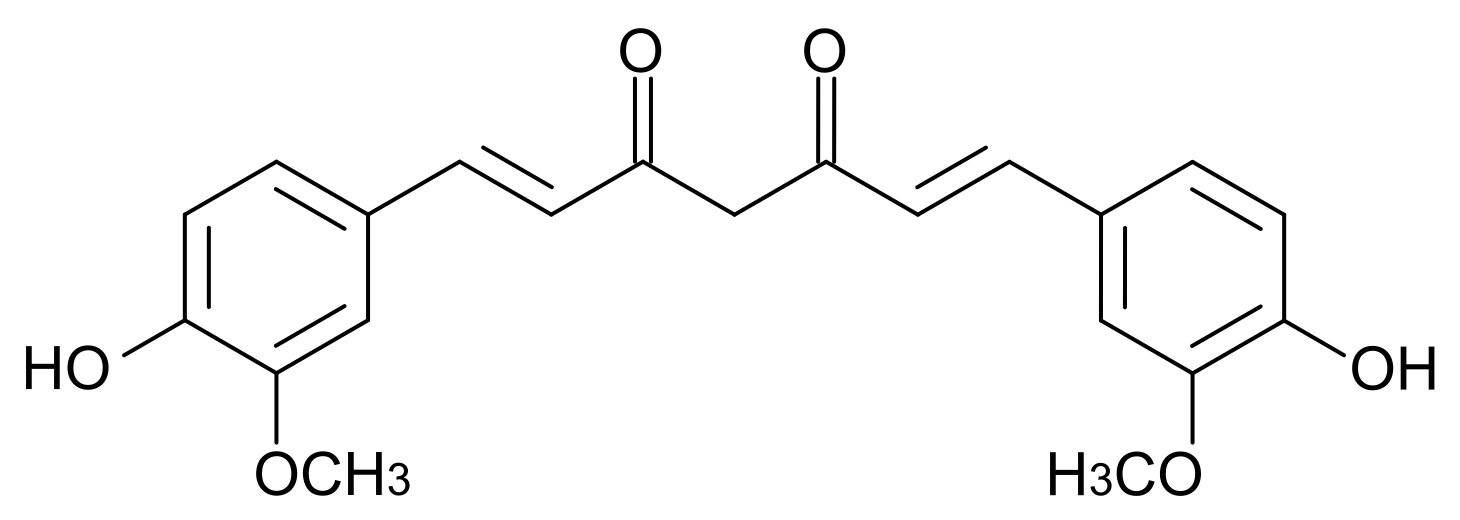
\includegraphics[width=.6\linewidth]{immagini/curcumina.png}
	\caption{Struttura molecolare della Curcumina.}
	\label{fig:curcumina}
\end{figure}

In questa sezione ci soffermeremo appunto sulla sintesi di un composto ottenuto fondendo alcune funzionalità della Curcumina con altre proprie del Donepezil, un farmaco la cui azione è mirata alla modulazione dell'azione dell'enzima AChE, ai fini di ottenere un possibile farmaco altamente affine alla permeazione della barriera emato-encefalica e con un'azione mirata nei confronti del substrato desiderato.

Le strutture dei composti d'interesse sono riportati in Figura \ref{fig:generale_curcdone} in si possono osservare i farmacofori della molecola di Curcumina (in rosso) e del Donepezil (in blu). Le funzionalità sono state collegate in maniera differente in modo da poter razionalizzare quale delle due serie (sempre mostrate in Figura \ref{fig:generale_curcdone}) presenti una migliore attività farmacologica. Diversi sostituenti sono stati impiegati per la medesima ragione; le funzionalità introdotte hanno lo scopo di regolare l'affinità per il substrato su cui agisce la molecola anche da un punto di vista dell'ingombro sterico.

\begin{figure}[H]
	\centering
	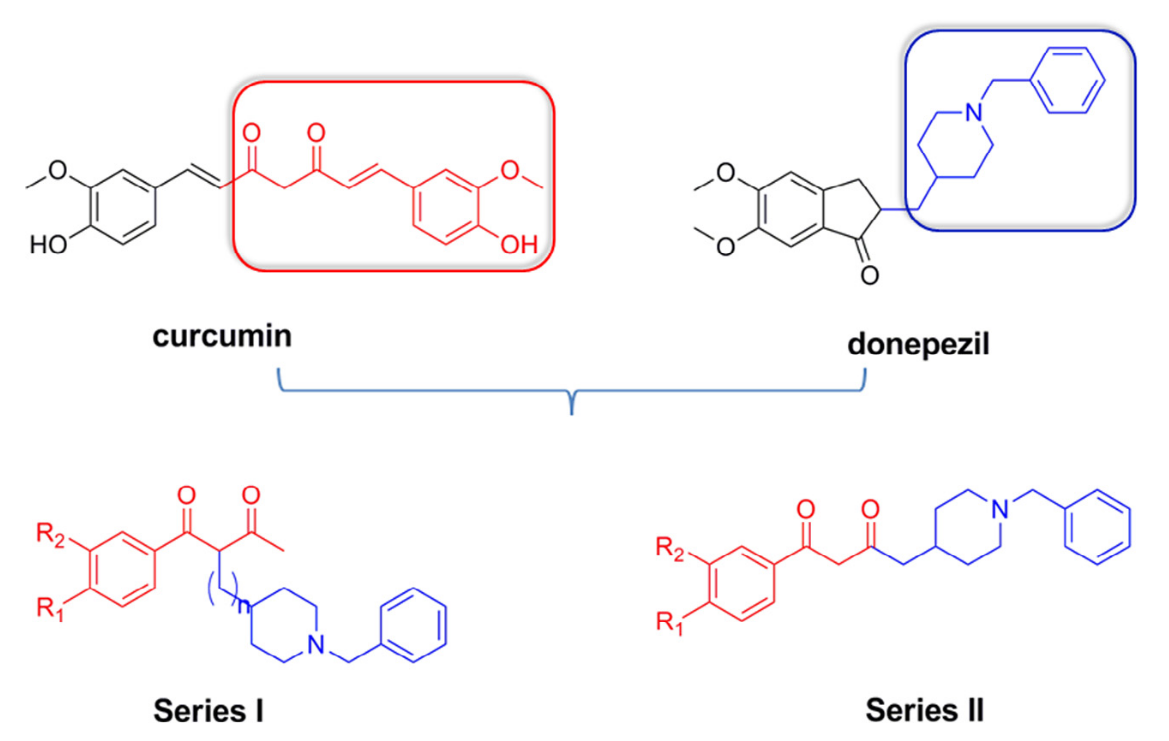
\includegraphics[width=\linewidth]{immagini/generale_curcdone.png}
	\caption{Formule di struttura dei composti ottenuti per fusione dei farmacofori appartenenti alla Curcumina (in rosso) e al Donepezil (in blu).}
	\label{fig:generale_curcdone}
\end{figure}



\subsection{Sintesi}
Il processo di sintesi per i composti d'interesse può essere scomposto nella sintesi dei farmacofori necessari; questi verranno poi accoppiati per formare i prodotti finali mediante condensazione aldolica.

\subsubsection{Sintesi del Farmacoforo del Donepezil}
\label{sec:sintesidone}
La reazione è rappresentata in maniera schematica in Figura \ref{fig:farmadone_curcdone}. A partire dai reagenti commerciali 1a-1b si effettua una reazione di Wittig in presenza di \ce{K2CO3} con l'intento di trasformare la funzione carbonilica in una esterea \(\alpha\),\(\beta\)-insatura. I prodotti 2a-2b ottenuti subiscono un processo di riduzione su Pd/C in modo da idrogenare il doppio legame formato nel passo precedente ma lasciando inalterate le insaturazioni del sistema aromatico.

I prodotti 3a-3b ottenuti possono essere isolati ed utilizzati come farmacofori del Donepezil per la sintesi dei composti della Serie II (si veda Sezione \ref{sec:condserie2}). Per la sintesi dei composti della Serie I sono necessari ancora due passaggi sintetici. In primis si riduce la funzione esterea ad alcool primario (composti 4a-4b) per mezzo di \ce{LiAlH4}, notare di nuovo come il processo di riduzione non tocchi l'anello aromatico presente nel substrato. Passaggio finale è l'ossidazione dell'alcool appena formato ad aldeide (composti 5a-5b); per fare ciò si esegue un'ossidazione di Swern. Tale processo ossidativo trova un'ottima applicazione in questo particolare caso in quanto l'alta tolleranza per quanto riguarda i gruppi funzionali permette l'ossidazione del sito d'interesse senza però in alcun modo intaccare altre porzioni della molecola. La reazione viene condotta utilizzando Cloruro di Ossarile, DMSO e Trietilammina. \autocite{bruice_chimica_2012}

\begin{figure}[H]
	\centering
	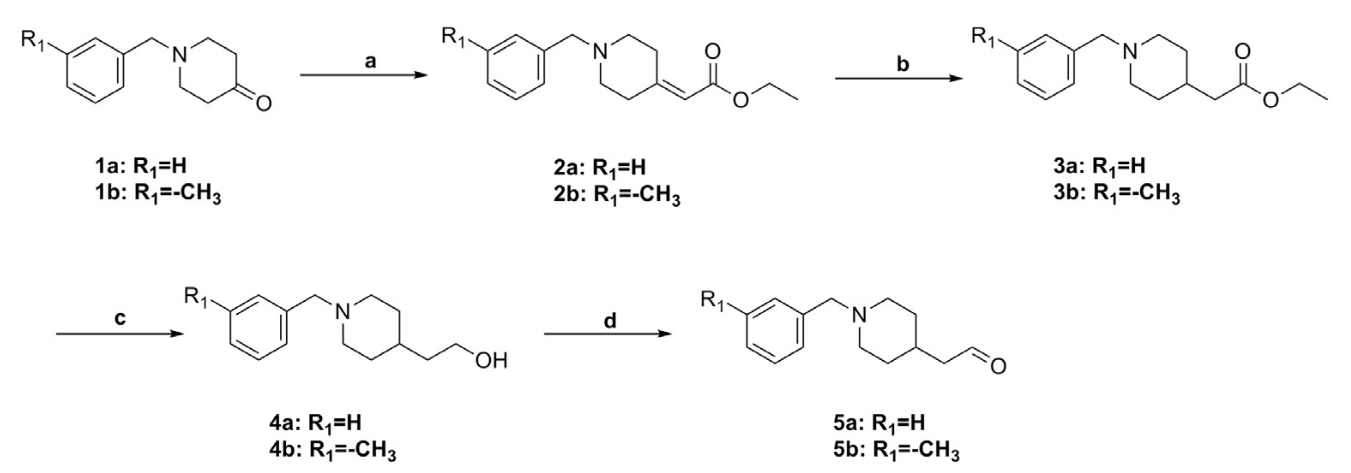
\includegraphics[width=\linewidth]{immagini/farmadone_curcdone.png}
	\caption{Passaggi sintetici per ottenere le due forme del farmacoforo del Donepezil: (a) \ce{(EtO)2POCH2CO2Et}, \ce{K2CO3} , THF; (b) Pd/C, \ce{H2} , \ce{MeOH}; (c) \ce{LiAlH4} , THF; (d) \ce{(COCl)2}, DMSO, \ce{N(CH2CH3)3}.}
	\label{fig:farmadone_curcdone}
\end{figure}

\subsubsection{Sintesi del Farmacoforo della Curcumina}
\label{sec:sintesicurc}
La sintesi della porzione di molecola corrispondente al farmacoforo della Curcumina è rappresentata in maniera schematica in Figura \ref{fig:farmacurc_curcdone}. I composti disponibili commercialmente 6a-6b vengono trattati con Diisopropiletilammina (DIPEA) e Cloruro di Metossimetiletere in Diclorometano al fine di proteggere la funzione idrossilica. I composti così ottenuti (7a-7b) assieme ad altri tre commercialmente disponibili (7c-7e) vengono trattati con Acetato di Etile in presenza di Ammoniuro di Sodio (\ce{NaNH2}) per ottenere i composti \(\beta\)-dichetone 8a-8e attraverso condensazione di Claisen.

Notare come la protezione con Metossimetiletere sia stata necessaria per evitare la deprotonazione dei siti idrossilici nel secondo passo reattivo per mano dell'Ammoniuro di Sodio.

Ai fini della sintesi dei composti d'interesse verranno utilizzati i prodotti 8a-8e per ottenere la prima serie di molecole, mentre i prodotti 7a, 7c e 7e  verranno sfruttati per ottenere la seconda serie.

\begin{figure}[H]
	\centering
	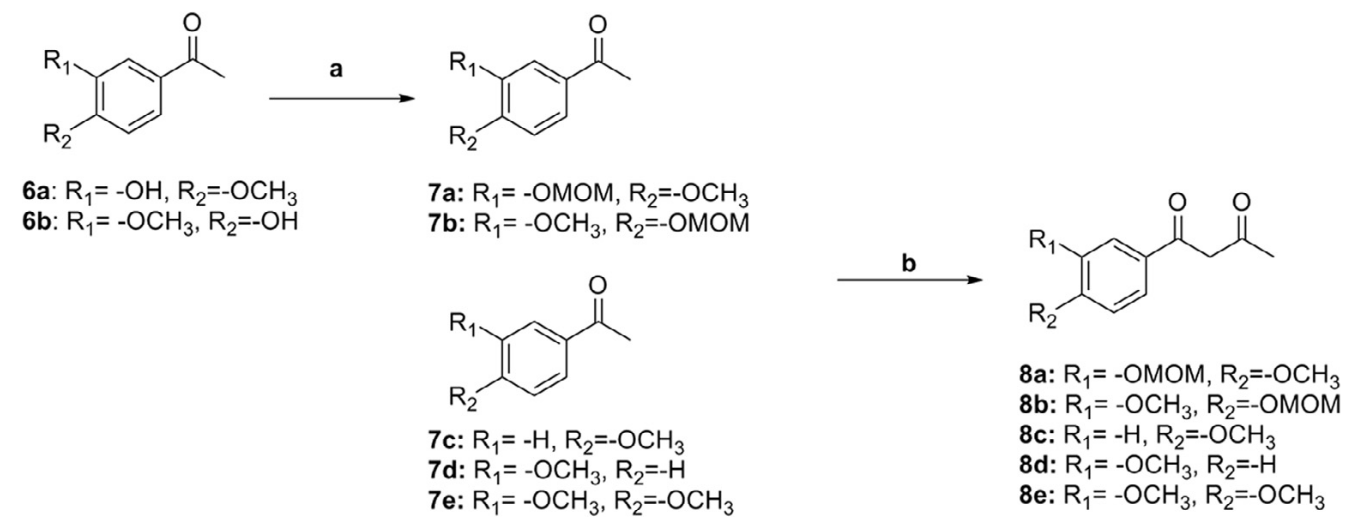
\includegraphics[width=\linewidth]{immagini/farmacurc_curcdone.png}
	\caption{Sintesi del farmacoforo della Curcumina: (a) \ce{MOMCl}, DIPEA, DCM; (b) \ce{NaNH2} , EtOAc, 60 $^\circ$C.}
	\label{fig:farmacurc_curcdone}
\end{figure}



\subsubsection{Sintesi dei Composti della Serie I}
\label{sec:condserie1}
La sintesi dei composti appartenenti alla prima serie è portata a termine in due passaggi sintetici riportati in Figura \ref{fig:condserie1_curcdone}; il primo è una condensazione aldolica effettuata a partire dalle aldeidi 5a-5b sintetizzate nella Sezione \ref{sec:sintesidone} ed il composto commerciale 9 con i \(\beta\)-dichetoni 8a-8e ottenuti come prodotto finale nella Sezione \ref{sec:sintesicurc}. La reazione viene condotta in presenza di quantità catalitiche di L-prolina, ai fini di fissare la stereochimica del nuovo legame formato, e di anidrificante \ce{MgSO4} in ambiente leggermente acido al fine di ottenere i relativi intermedi \(\alpha\),\(\beta\)-insaturi (non rappresentati in Figura). Questi	vengono ridotti nel secondo passaggio sintetico per mezzo di una reazione di riduzione Pd/C catalizzata dopo la quale è possibile isolare i prodotti finali 10a-10l.

Un ulteriore passaggio sintetico viene eseguito sui composti che presentano la protezione metossimetileterea, questa viene rimossa ripristinando la funzione idrossilica con un semplice trattamento con HCl e EtOH.

\begin{figure}[H]
	\centering
	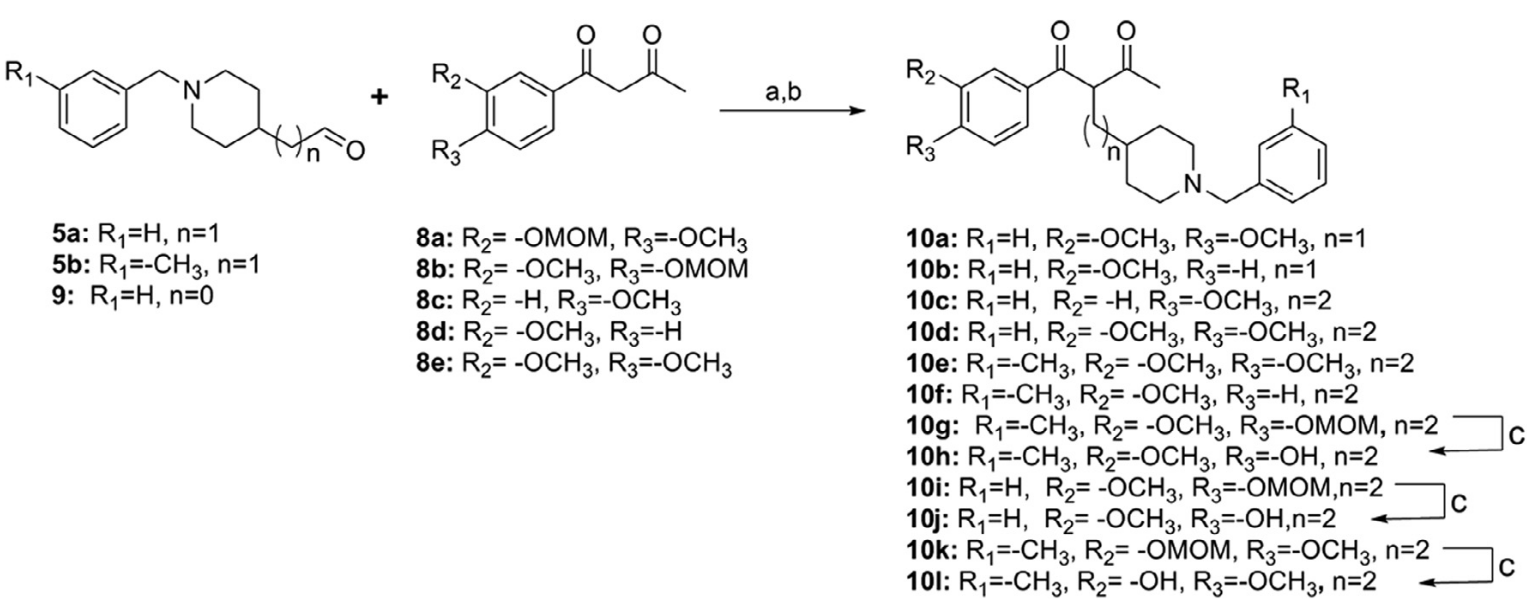
\includegraphics[width=\linewidth]{immagini/condserie1_curcdone.png}
	\caption{Sintesi dei composti d'interesse appartenenti alla Serie I: (a) L-prolina, \ce{MgSO4} , EtOH, reflusso; (b) 10\% Pd/C, MeOH; (c) HCl, EtOH.}
	\label{fig:condserie1_curcdone}
\end{figure}

\subsubsection{Sintesi dei Composti della Serie II}
\label{sec:condserie2}
La seconda serie di composti è sintetizzata come indicato in Figura \ref{fig:condserie2_curcdone}; una condensazione di Claisen tra i composti 7a, 7c e 7e ottenuti come intermedi isolabili nella Sezione \ref{sec:sintesicurc} e i composti 3a-3b anch'essi intermedi isolati nel processo sintetico presentato nella Sezione \ref{sec:sintesidone}.

Come per i composti della prima serie una reazione successiva rimuove la deprotezione metilmetossieterea nei composti che la presentano.

\begin{figure}[H]
	\centering
	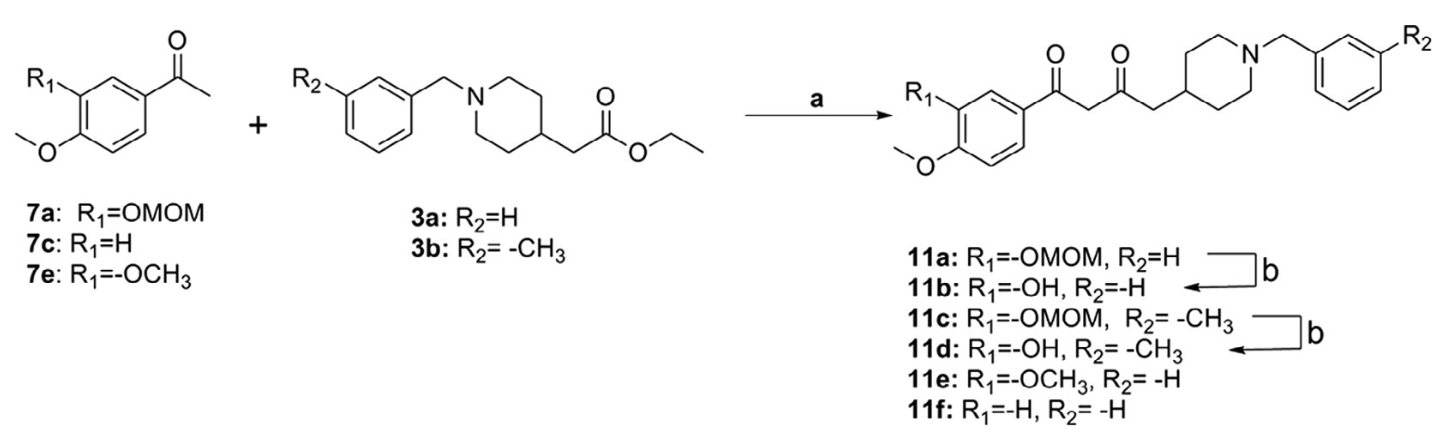
\includegraphics[width=\linewidth]{immagini/condserie2_curcdone.png}
	\caption{Sintesi dei composti d'interesse appartenenti alla Serie II: (a) \ce{NaNH2} , THF, 60 $^\circ$C; (b) HCl, EtOH.}
	\label{fig:condserie2_curcdone}
\end{figure}

\subsection{Effetti delle Molecole Sintetizzate}
Innanzitutto è stato studiato l'effetto d'inibizione dei vari composti sintetizzati ai fini di determinare quali fossero potenzialmente adatti per un uso terapeutico; l'indagine è stata effettuata osservando in vitro l'effetto delle molecole ottenute sull'attività dell'enzima AChE usando come parametro di riferimento l'azione di Tacrina, noto inibitore reversibile dell'enzima in questione, Donepezil e Galantamina, due farmaci riconosciuti per la loro azione inibitrice dell'AChE. È stata anche valutata la selettività d'inibizione verificando l'azione degli stessi composti su di un altro enzima (BuChE) la cui attività non necessita di modulazione per il trattamento di pazienti affetti da AD. I risultati sono riportati in Figura \ref{fig:tabellacomposti_curcdone}.

\begin{figure}[H]
	\centering
	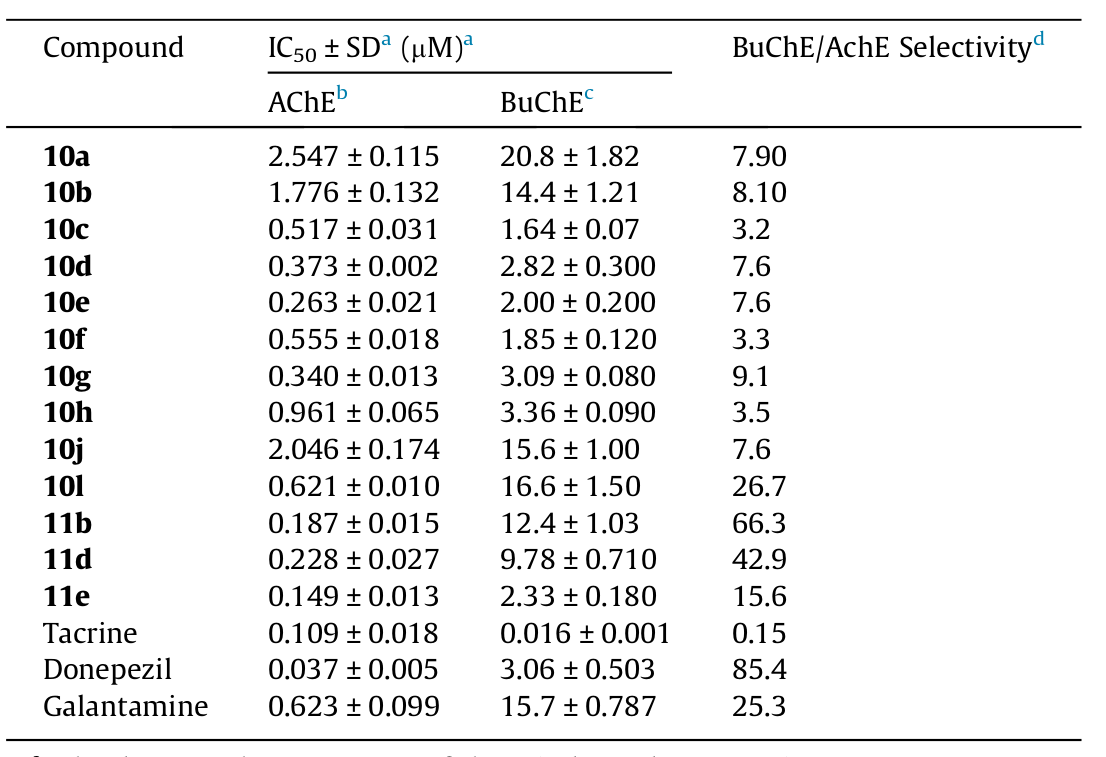
\includegraphics[width=.8\linewidth]{immagini/tabellacomposti_curcdone.png}
	\caption{Azione d'inibizione sull'enzima AChE. (a) La deviazione standard è riferita a tre esperimenti indipendenti effettuati; (b) enzima AChE ottenuto da Murena Helena; (c) enzima BuChE ottenuto da siero equino; (d) selettività espressa come rapporto degli IC\textsubscript{40} per i due enzimi.}
	\label{fig:tabellacomposti_curcdone}
\end{figure}

Dai risultati sono possibili alcune considerazioni sulle relazioni struttura-attività:

\begin{enumerate}
	\item Per i composti della Serie I una lunghezza della catena di atomi di carbonio tra il dichetone e il sostituente piridinico di 2 ha comportato un aumento dell'azione inibitoria.
	\item Se la catena ha invece lunghezza 1 (composti 10a-10c) la presenza di un gruppo metossile in posizione para ha dimostrato migliore inibizione nei confronti del AChE (composto 10c).
	\item La presenza di un gruppo metilico in posizione R\textsubscript{3} ha mostrato un miglioramento dell'attività.
	\item Sempre in posizione R\textsubscript{3} il gruppo idrossile ha dimostrato un'attività peggiore del gruppo idrossilico (confronto tra 10d e 10j, 10e e 10h).
	\item I composti appartenenti alla Serie II (11b, 11d e 11e) hanno mostrato una più forte inibizione ed una migliore selettività di quelli appartenenti alla Serie I.
	\item La migliore selettività è stata dimostrata dal composto 11b anche se inferiore rispetto al semplice Donepezil preso di riferimento.
\end{enumerate}

Risulta quindi chiaro come le molecole appartenenti alla seconda serie risultino essere i migliori candidati tra quelle sintetizzate; esse sono quindi studiate in maniera più approfondita valutando altri fattori che potrebbero indicare una buona azione in pazienti affetti da AD.

Una delle fondamentali proprietà necessarie affinché le molecole possano avere applicazioni in campo medico è la permeabilità della barriera emato-encefalica. Tutti e tre i composti della seconda serie (11b, 11d e 11e) hanno presentato valori di permeabilità ottimi mostrando quindi lo stesso comportamento della Curcumina utilizzata come base strutturale.

Un altra delle proprietà studiate è la capacità antiossidante; come nel caso del Resveratrolo affrontato nella Sezione \ref{effetti_resveratrolo} uno dei benefici dell'impiego dei polifenoli come medicinali in pazienti affetti da AD è la capacità di questa classe di molecole di diminuire la concentrazione di ROI nell'organismo. Per valutare gli effetti dei composti 11b, 11d e 11e sono stati condotti in vitro alcuni esperimenti utilizzando una fluoresceina come nel caso del Resveratrolo per evidenziare la presenza di specie perossidiche. Come riferimento è stato usato il Trolox, analogo della vitamina E. I risultati ottenuti sono riportati in Figura \ref{fig:roi_curcdone} come equivalenti di Trolox. Tutti e tre i composti hanno mostrato un discreto effetto di riduzione di specie ROI con un risultato degno di nota nel caso del composto 11b, tale comportamento è legato alla presenza del gruppo ossidrilico in posizione meta in grado di "spegnere" i radicali dannosi generati.

\begin{figure}[H]
	\centering
	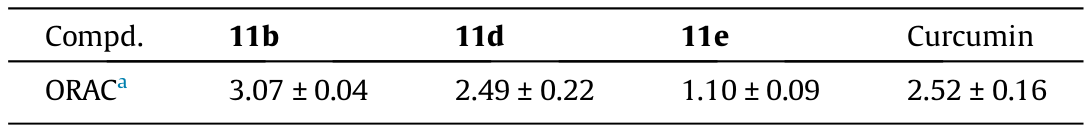
\includegraphics[width=\linewidth]{immagini/roi_curcdone.png}
	\caption{Attività antiossidante dei composti 11b, 11d e 11e rispetto alla Curcumina. I valori riportati sono espressi in equivalanti/$\mu$mol di Trolox. (a) La deviazione standard è riferita a tre esperimenti indipendenti effettuati.}
	\label{fig:roi_curcdone}
\end{figure}


L'ultimo dei fattori presi in esame è la capacità delle molecole di inibire l'aggregazione dei frammenti A\(\beta\) sia in presenza che in assenza di ioni metallici.

L'aggregazione in assenza di metalli è stata valutata attraverso lo spettro di fluorescenza in presenza di Tioflavina T (ThT). I composti 11b, 11d e 11e sono stati confrontati con l'azione della curcumina in concentrazioni pari a 20 $\mu$M. I risultati riportati in Figura \ref{fig:selfab_curcdone} mostrano un discreto effetto inibitorio soprattutto in presenza di un gruppo ossidrile e di basso ingombro sterico (composto 11b).

\begin{figure}[H]
	\centering
	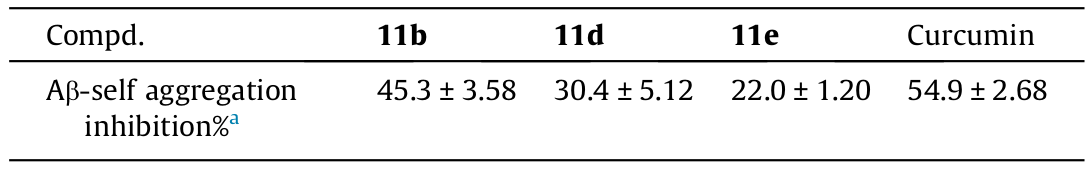
\includegraphics[width=\linewidth]{immagini/selfab_curcdone.png}
	\caption{Inibizione dell'aggregazione dei A\(\beta\) in assenza di metalli. (a) La deviazione standard è riferita a tre esperimenti indipendenti effettuati.}
	\label{fig:selfab_curcdone}
\end{figure}

In presenza di metalli, come abbiamo già introdotto nella Sezione \ref{sec:ab}, la formazione degli aggregati proteici è legata alla concentrazione di ioni metallici liberi. La capacità di chelare tali ioni è quindi il fattore da valutare. Il composto preso in considerazione è l'11b visti gli ottimi risultati ottenuti nei precedenti esperimenti per la valutazione della sua efficacia. Lo studio sull'aggregazione è effettuabile confrontando gli spettri UV-vis del composto in assenza di metallo e dopo l'aggiunta in soluzione di \ce{CuSO4}, uno spostamento della lunghezza d'onda d'assorbimento evidenzia la formazione del complesso 11b-Cu(II). Lo stesso esperimento è stato condotto in presenza di \ce{FeSO4} e \ce{ZnCl2}; i risultati sono riportati in Figura \ref{fig:metab_curcdone}. In presenza di Fe(II) e di Cu(II) si è osservato il fenomeno di chelazione mentre non sono stati osservati effetti rilevanti per lo Zinco. \autocite{jun_yan_design_2017}

\begin{figure}[H]
	\centering
	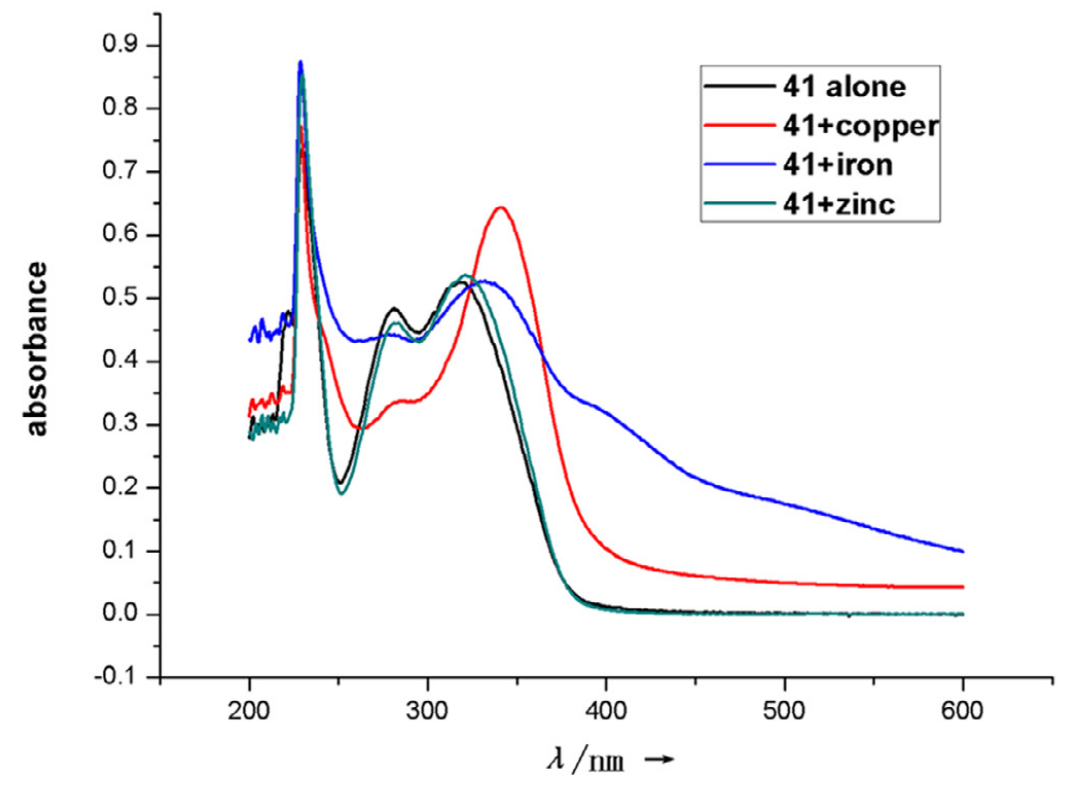
\includegraphics[width=\linewidth]{immagini/metab_curcdone.png}
	\caption{Spettro UV-vis per il composto 11b in presenza o meno di ioni metallici.}
	\label{fig:metab_curcdone}
\end{figure}


\section{Leganti Bipiridinici}
\label{sec:byp}
Andiamo ora a considerare una classe di composti la cui azione principale non è legata alla regolazione dell'attività ormonale ma ad una mitigazione del fenomeno d'aggregazione in placche dei A\(\beta\). Come presentato nella Sezione \ref{sec:ab} uno dei meccanismi di aggregazione considerati alla base della formazione degli agglomerati proteici neurotossici prevede che il formarsi di un complesso tra metalli in concentrazioni sopra la norma nel liquido cerebrospinale e i A\(\beta\) stessi.

L'idea alla base di un trattamento agente su questo meccanismo prevede una diminuzione dei metalli biodisponibili attraverso una chelazione degli stessi per mezzo di leganti organici.

\subsection{Le Molecole}
\label{sec:bpy_mol}
Per progettare una molecola in grado di svolgere il compito appena descritto occorrerà che questa soddisfi alcuni criteri:
\begin{enumerate}
	\item Capacità di complessare il metallo d'interesse.
	\item Costanti d'equilibrio elevate per quanto riguarda la forma complessata.
	\item Buona solubilità in ambiente acquoso, in modo da permettere la diffusione del composto all'interno del corpo.
	\item Buona permeabilità della barriera emato-encefalica; un composto che non soddisfi questo criterio avrà difficoltà ad essere trasferito nel liquido cerebrospinale.
\end{enumerate}
Una classe di composti le cui proprietà soddisfano i criteri appena presentati è quella dei derivati bipiridinici (Figura \ref{fig:bpy}).
Questi presentano una chelazione veloce, ovvero con k\textsubscript{f} nei confronti dei metalli d'interesse (Cu(II) e Zn(II)) di circa 7.0, grazie alla chelazione dell'atomo metallico da parte degli atomi d'azoto nei due eterocicli. Inoltre la solubilità in medium acquosi è relativamente buona, stiamo parlando di circa 5,9 mg/mL; infine le dimensioni ridotte permettono una buona diffusione nel sistema nervoso permeando attraverso la barriera emato-encefalica con discreta facilità (i valori di permeabilità possono essere stimati attraverso le regole empiriche di Lipinski o attraverso test in vitro). \autocite{di_high_2003}
\begin{figure}[H]
	\centering
	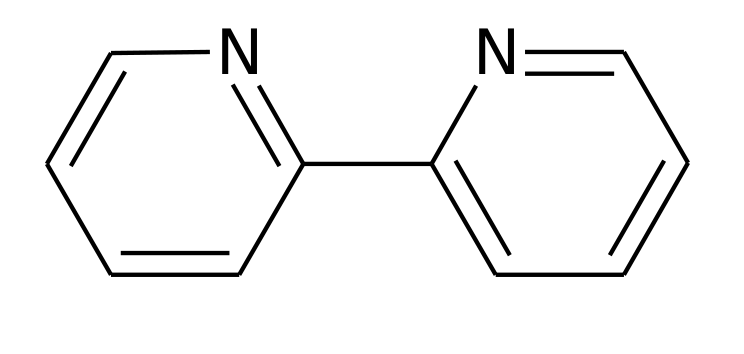
\includegraphics[width=.5\linewidth]{immagini/bpy.png}
	\caption{Un generico composto appartenente alla classe delle Bipiridine.}
	\label{fig:bpy}
\end{figure}
Lo scheletro bipiridinico ben si presta ad un approccio razionale nella sintesi di composti interessanti dal punto di vista biomedico.
L'introduzione di gruppi dimetilamminici favorisce un'interazione con i A\(\beta\) e per la sua influenza sul legame metallico come suggerito da alcune evidenze sperimentali. Similmente l'uso di un sostituente metilico permette un migliore effetto elettrodonatore da parte degli eteroatomi nei cicli e un controllo sterico sui possibili orientamenti con cui la molecola bipiridinica può interagire con il metallo. \autocite{derrick_importance_2016,savelieff_ongoing_2014}

Ai fini di dimostrare l'effetto di queste modificazioni a partire dalla struttura di base sull'azione di inibizione alla formazione e disfacimento di placche amiloidiche useremo quattro prodotti di sintesi, presentati nella loro struttura in Figura \ref{fig:bpy_mod}; nella sezione successiva andremo quindi a presentare un possibile processo sintetico per essi.

\begin{figure}[H]
	\centering
	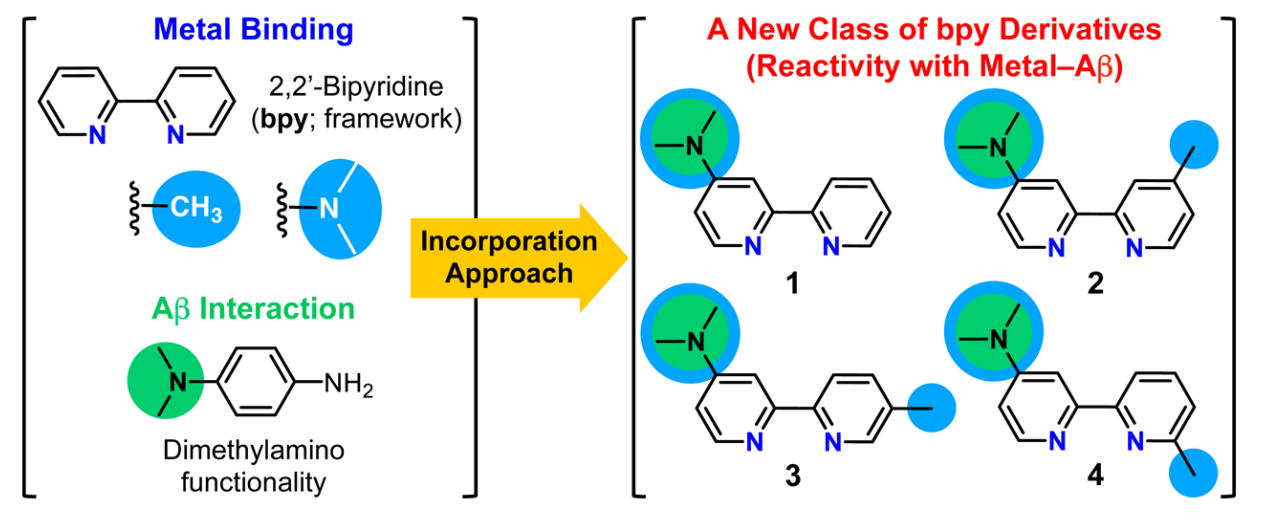
\includegraphics[width=\linewidth]{immagini/bpy_mod.png}
	\caption{Funzionalità introdotte sullo scheletro bipiridinico ai fini di ottenere i composti d'interesse 1-4}
	\label{fig:bpy_mod}
\end{figure}

\subsection{Sintesi}
\label{sec:bpy_stille}
Il processo di sintesi utilizzato è riassunto in maniera sintetica nella Figura \ref{fig:rea_g}; a partire da una 4-amminopiridina si ottiene un composto organometallico allo stagno; successivamente per mezzo di una reazione di Stille si addiziona il primo anello al secondo ottenendo il prodotto desiderato.

Un metodo alternativo per la sintesi di questi composti bipiridinici potrebbe essere la reazione di accoppiamento di Negishi. Si tratta sempre di una reazione di accoppiamento ma tra un composto organozinco, invece di uno stannano, e un alogenuro, nel nostro caso una piridina alogenata. \autocite{clayden_organic_2012}

A differenza della Reazione di Stille proposta, in cui l'accoppiamento viene promosso da un composto organostannano, l'uso di Zinco, la cui tossicità è nota per essere inferiore rispetto a quella dello Stagno. Il maggiore inconveniente della reazione di accoppiamento di Negishi è la sensibilità all'esposizione all'aria e all'acqua oltre ad una minore tolleranza circa il tipo di gruppi funzionali con cui è possibile lavorare per cui la Stille rimane la scelta preferibile in questo caso. \autocite{nicolaou_palladium-catalyzed_2005}

\begin{figure}[H]
	\centering
	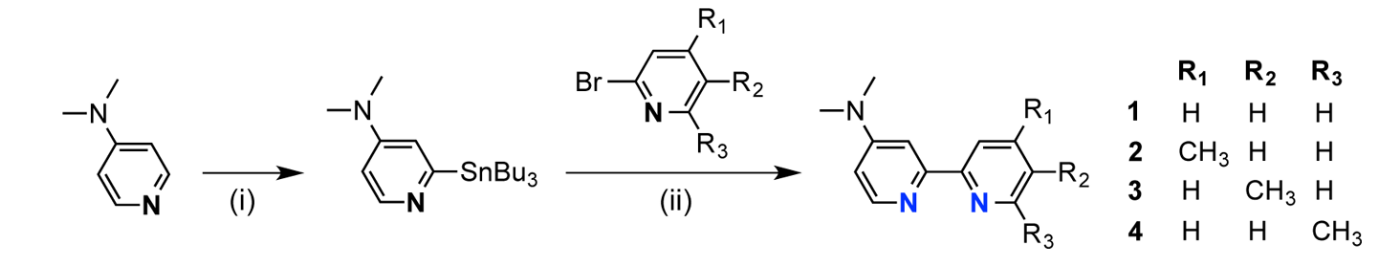
\includegraphics[width=\linewidth]{immagini/rea_g.png}
	\caption{Reazione generale per l'ottenimento dei composti d'interesse 1-4. (i) n-BuLi, 2-Dimetilaminoetanolo, Esano, 0 $^\circ$C; \ce{Bu3SnCl}, -78 $^\circ$C; (ii) \ce{PdCl2(PPh3)2}, \ce{LiCl}, \ce{PPh3}, Toluene, 110 $^\circ$C }
	\label{fig:rea_g}
\end{figure}

\subsubsection{Reazione di Formazione dello Stannano }
Il reagente di partenza, ovvero la 4-dimetilamminopiridina, viene trattata con \ce{n-BuLi} al fine di deprotonare la posizione 2 rispetto all'atomo di azoto presente nell'anello. Lo stannano è ottenuto per transmetallazione dell'organolitiato; il \ce{Bu3SnCl} reagisce con il substrato sostituendosi all'atomo di \ce{Li} il quale si lega al \ce{Cl}.

È importante notare come la soluzione venga mantenuta a basse temperature (-78 $^\circ$C) affinché la reazione di deprotonazione abbia luogo nel sito desiderato e che il composto organolitiato ottenuto sia sufficientemente stabile in modo tale da permettere la sostituzione con lo Stagno.

\subsubsection{Reazione di Stille per Formazione del Prodotto Finale}
Il secondo passaggio per l'ottenimento dei composti bipiridinici d'interesse prevede una reazione di Stille, ovvero una reazione di cross-coupling palladio-catalizzata, nel caso particolare preso in esame, tra lo stannano ottenuto come prodotto dello step di reazione precedente e un alogenuro alchilico piridinico.\autocite{clayden_organic_2012}

Il processo catalitico generale è riportato in maniera schematica in Figura \ref{fig:stille}.

\begin{figure}[H]
	\centering
	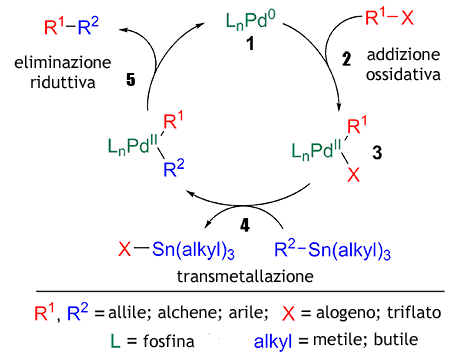
\includegraphics[width=.9\linewidth]{immagini/stille.png}
	\caption{Rappresentazione schematica del ciclo catalitico coinvolto in una reazione di Stille. Nel caso in esame R\textsuperscript{1}=2-bromopiridina, 2-bromo-4-metilpiridina, 2-bromo-5-metilpiridina, 2-bromo-6-metilpiridina R\textsuperscript{2}=N,N-dimetil-2-(tributilstannil)-piridin-4-ammina.}
	\label{fig:stille}
\end{figure}

In Toluene sono introdotti lo stannano, prodotto di reazione del passaggio sintetico precedente, il catalizzatore al palladio \ce{PdCl2(PPh3)2}, Trifenilfosfina e Cloruro di Litio. A seconda del composto bipiridinico desiderato come prodotto finale viene infine introdotta l'appropriata piridina bromurata.

Il ciclo catalitico può essere riassunto in cinque passaggi:
\begin{enumerate}
	\item Il catalizzatore \ce{PdCl2(PPh3)2} viene ridotto a \ce{Pd(PPh3)2}, un complesso a 14 elettroni in cui il Pd ha stato d'ossidazione 0.
	\item Il complesso subisce addizione ossidativa da parte dell'alogenuro: si tratta di un processo concertato che forma un complesso a 16 elettroni con i due nuovi leganti in posizione cis.
	\item Si osserva un equilibrio d'isomerizzazione tra la forma cis e trans del complesso organometallico. La forma trans è favorita dal punto di vista termodinamico visto l'ingombro sterico originato dai leganti \ce{PPh3}.
	\item Si ha transmetallazione tra lo stannano in soluzione ed il complesso; il risultato è il trasferimento del composto arilico sul complesso con allontanamento dell'alogenuro.
	\item Un processo di eliminazione riduttiva libera il composto bipiridinico ripristinando il catalizzatore; da qui il ciclo ricomincia.
\end{enumerate}

La reazione viene condotta sotto atmosfera inerte d'Azoto per evitare che il catalizzatore possa essere alterato dalle componenti dell'aria.

\subsection{Effetti delle Molecole Sintetizzate sui A\(\beta\)}
L'efficacia dei composti ottenuti rispetto all'aggregazione dei A\(\beta\) è stata quantificata attraverso esperimenti in vitro. I risultati sono riportati nella Figura \ref{fig:ris_bpy} per quanto riguarda l'azione in presenza di A\(\beta\)-40 e nella Figura \ref{fig:ris_bpy2} per il caso di A\(\beta\)-42.

\begin{figure}[H]
	\centering
	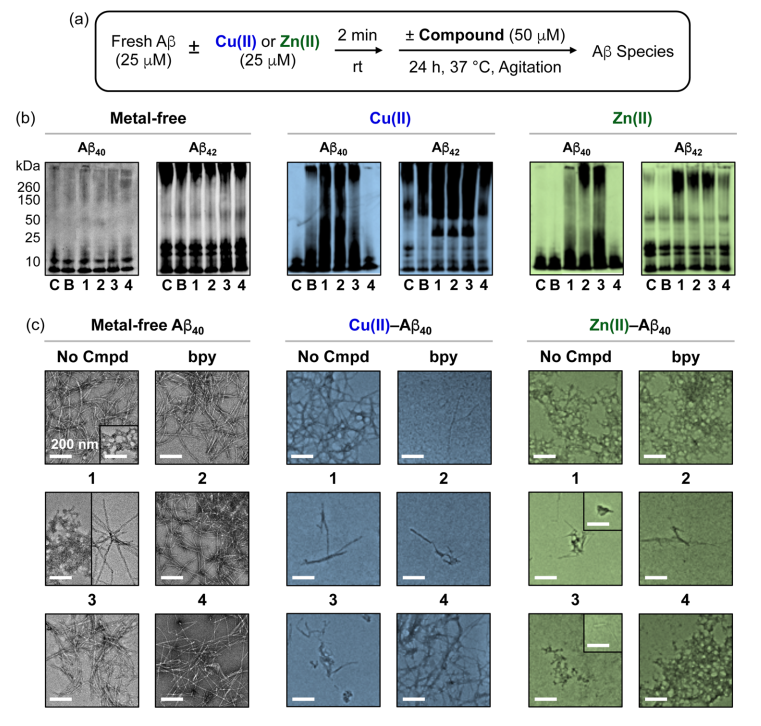
\includegraphics[width=\linewidth]{immagini/ris_bpy.png}
	\caption{(a) schematica rappresentazione della metodologia di sperimentazione; (b) corse elettroforetiche per la visualizzazione della dimensionalità delle specie A\(\beta\)\-40 e A\(\beta\)\-42 per mezzo di tecnica immunofissativa \autocite{kurien_western_2006}; (c) immagini ottenute al microscopio elettronico a trasmissione (TEM) dai campioni incubati per 24 ore. C=A\(\beta\)+M, B=C+bpy, 1=C+1, 2=C+2, 3=C+3, 4=C+4 }
	\label{fig:ris_bpy}
\end{figure}

\begin{figure}[H]
	\centering
	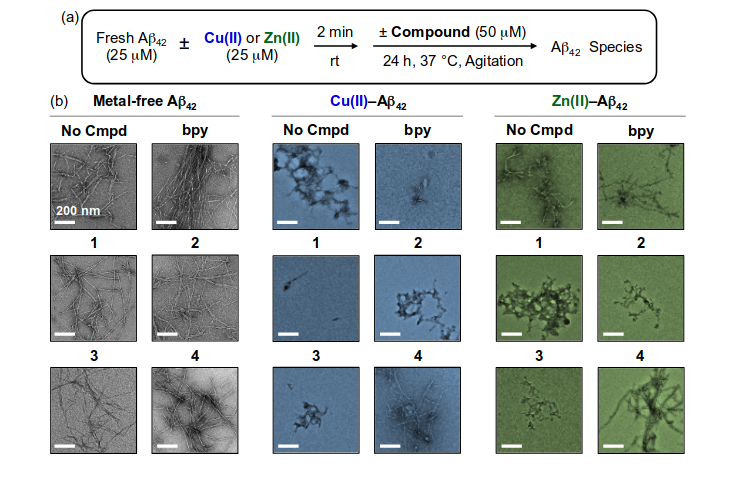
\includegraphics[width=\linewidth]{immagini/ris_bpy2.png}
	\caption{(a) schematica rappresentazione della metodologia di sperimentazione; (b) immagini ottenute al microscopio elettronico a trasmissione (TEM) dai campioni incubati per 24 ore. C=A\(\beta\)+M, B=C+bpy, 1=C+1, 2=C+2, 3=C+3, 4=C+4 }
	\label{fig:ris_bpy2}
\end{figure}

Nelle corse elettroforetiche mostrate in Figura \ref{fig:ris_bpy}, sezione (b), si osserva come la dimensione degli aggregati proteici tenda a diminuire in presenza dei composti sintetizzati agenti su soluzioni contenenti ioni metallici, mentre in assenza di un centro di nucleazione metallico non vi siano apprezzabili effetti di mitigazione dell'accrescimento della placca. Questo è un dato atteso, i composti progettati hanno infatti lo specifico compito di chelare metalli per diminuire il fenomeno d'aggregazione, logico quindi osservare come in assenza di ioni non vi siano benefici evidenti.

Soffermandoci sulle immagine ottenute al TEM possiamo vedere come l'azione del semplice scheletro bipiridinico (bpy) modifichi l'aggregazione in presenza di Cu(II) ma non abbia evidenti effetti se confrontata con il campione C in presenza di Zn(II). I composti sintetizzati senza gruppo metilico (1) e quelli con il gruppo metilico in posizioni meta o para (2 e 3) hanno invece inibito la formazione di conglomerati di A\(\beta\)\-40 e A\(\beta\)\-42 sia in presenza di Cu(II), sia di Zn(II).

Il composto 4, ovvero quello con il gruppo metilico in posizione orto non ha alterato l’aggregazione dei filamenti proteici in nessuna delle situazioni ricreate in vitro. Si tratta di un risultato atteso in quanto l’ingombro sterico del gruppo \ce{CH3} impedisce la chelazione del metallo libero che può quindi risultare disponibile come centro di nucleazione.

Benché le molecole sintetizzate risultino efficaci nella chelazione dei metalli liberi responsabili dell’accrescimento dei grumi di A\(\beta\) e che la loro capacità di permeare la barriera necessaria per entrare in circolazione nel liquido cerebrospinale sia confermata da evidenze scientifiche (come già evidenziato nella Sezione \ref{sec:bpy_mol}), un test della tossicità su cellule di tipo Y5 ha evidenziato livelli notevoli di citotossicità in situazioni di concentrazioni millimolari di Rame(II), stimolando quindi Apoptosi neuronale e vanificando quindi la possibilità di un'azione diretta come farmaco dei composti in questione.

È comunque importante considerare i risultati ottenuti, si è infatti osservato come la diminuzione degli ioni metalli biodisponibili sia un metodo efficace (almeno in vitro) per limitare l'aggregazione in fibrille dei A\(\beta\) e che quindi la ricerca di composti la cui tossicità per l'organismo sia inferiore pur mantenendo simili proprietà possa essere una via promettente per il futuro. \autocite{ji_strategic_2017}

\section{Conclusioni}
In conclusione, la ricerca di una cura al morbo d'Alzheimer è un campo ancora molto aperto; le ipotesi circa le cause che comportano il presentarsi della patologia sono tante e non completamente chiare.\ In questo lavoro di tesi mi sono soffermato soltanto su una delle tante sfaccettature del mondo della ricerca in questo campo. Soltanto attraverso un lavoro congiunto multidisciplinare si è riusciti ad ottenere i risultati presentati in queste pagine; il ruolo del chimico organico è quello di fornire a medici, biochimici e biotecnologi gli strumenti, sotto forma di molecole, per poter indagare in maniera più profonda il problema dell'Alzheimer e di poter individuare una cura efficace che purtroppo ad oggi non è stata ancora individuata.

I tre casi che sono stati presentati sono appunto un esempio di ciò che la chimica organica può offrire nel tentativo di individuare una possibile cura: usando molecole naturali come base per la sintesi di composti ad esse ispirati in grado di permeare la barriera emato-encefalica e fornire effetti antiossidanti e/o di limitare l'aggregazione proteica come nel caso di Resveratrolo e Curcumina; oppure realizzando tramite un approccio razionale alla sintesi molecole ad hoc in grado di avere gli effetti desiderati sull'organismo come i composti bipiridinici presentati.

\newpage

\section{Ringraziamenti}
Un sentito ringraziamento va prima di tutto alla mia relatrice, la Professoressa Annamaria Deagostino, per il supporto fornito in fase di stesura di questo elaborato e per la passione trasmessami per la chimica organica.

Un dovuto ringraziamento alla mia famiglia senza la quale nulla di tutto questo sarebbe stato possibile. Un immenso ringraziamento alla mia compagna Beatrice che ha saputo sopportarmi anche nei momenti più bui e pieni d'incertezze. Un grande grazie al mio compagno di studi Fabio senza cui probabilmente non avrei trovato la forza di studiare per alcuni esami per me particolarmente ostici. Grazie a tutti i miei colleghi che hanno reso meno pesanti le giornate in ateneo anche solo con un sorriso sincero ed una stretta di mano. Grazie a tutti.




\newpage

\printbibliography

\end{document}
